\section{Adiabatic Basis}
\label{sec:adiabatic-basis}


The matrix form of the Hamiltonian in the rotated frame takes the form:
\begin{equation}
    H(t) = \frac{1}{2}
    \begin{bmatrix}
            -\Delta & \Omega(t) \\ \Omega(t)  & \Delta
    \end{bmatrix}
\label{eq:rotated-hamiltonian-matrix}
.\end{equation}

The Rabi frequency $\Omega(t)$ quantifies the field-induced coupling between the two states. The instantaneous eigenstates of \( H(t) \), commonly referred to as the adiabatic states, are:
\begin{align}
| w_- (t) \rangle &= \cos \vartheta(t) |0\rangle - \sin \vartheta(t) |1\rangle, \\
| w_+ (t) \rangle &= \sin \vartheta(t) |0\rangle + \cos \vartheta(t) |1\rangle
\label{eq:rotating_basis}
,\end{align}
where the mixing angle is given by  $\vartheta(t) = \frac{1}{2}\arctan\frac{\Omega(t)}{\Delta}$. The corresponding eigenvalues, representing the adiabatic energy levels, are:
\begin{equation}
\varepsilon_{\pm}(t) = \frac{\hbar}{2} \left( \Delta \pm \sqrt{\Omega^2(t) + \Delta^2} \right)
,\end{equation}
yielding an energy gap of $\varepsilon(t) =\varepsilon_+(t) - \varepsilon_-(t) = \hbar \sqrt{\Omega^2(t) + \Delta^2}$.

Using the eigenvectors from Eq. (\ref{eq:rotating_basis}) we define the adiabatic transformation matrix $R$. Applying this transformation to the Hamiltonian in Eq. (\ref{eq:rotated-hamiltonian-matrix}) gives the  Hamiltonian in the adiabatic basis $H^{a} = R^{\dagger} H R - i R^{\dagger} \dot{R}$, which can be explicitly written as:



\begin{equation}
    H^a(t) = \frac{1}{2}
    \begin{bmatrix}
            -\varepsilon(t)/2 & -i\dot{\vartheta}(t) \\ \dot{\vartheta}(t)  & \varepsilon(t)/2
    \end{bmatrix}
    .
\end{equation}
Adiabatic evolution requires that the rate of change of the mixing angle \( \vartheta(t) \) is much smaller than the energy splitting $\varepsilon(t)$, leading to the adiabatic condition \cite{boradjiev_power_2013}:
\begin{equation}
| 2\dot{\vartheta}| \ll \varepsilon(t),
\label{eq:adiabatic-condition}
\end{equation}
where the non-adiabatic coupling term is given explicitly by $| \dot{\vartheta}| = \frac{\Delta\dot{\Omega}(t)}{2[\Delta+\Omega(t)]}$. 



\begin{figure}
    \centering
    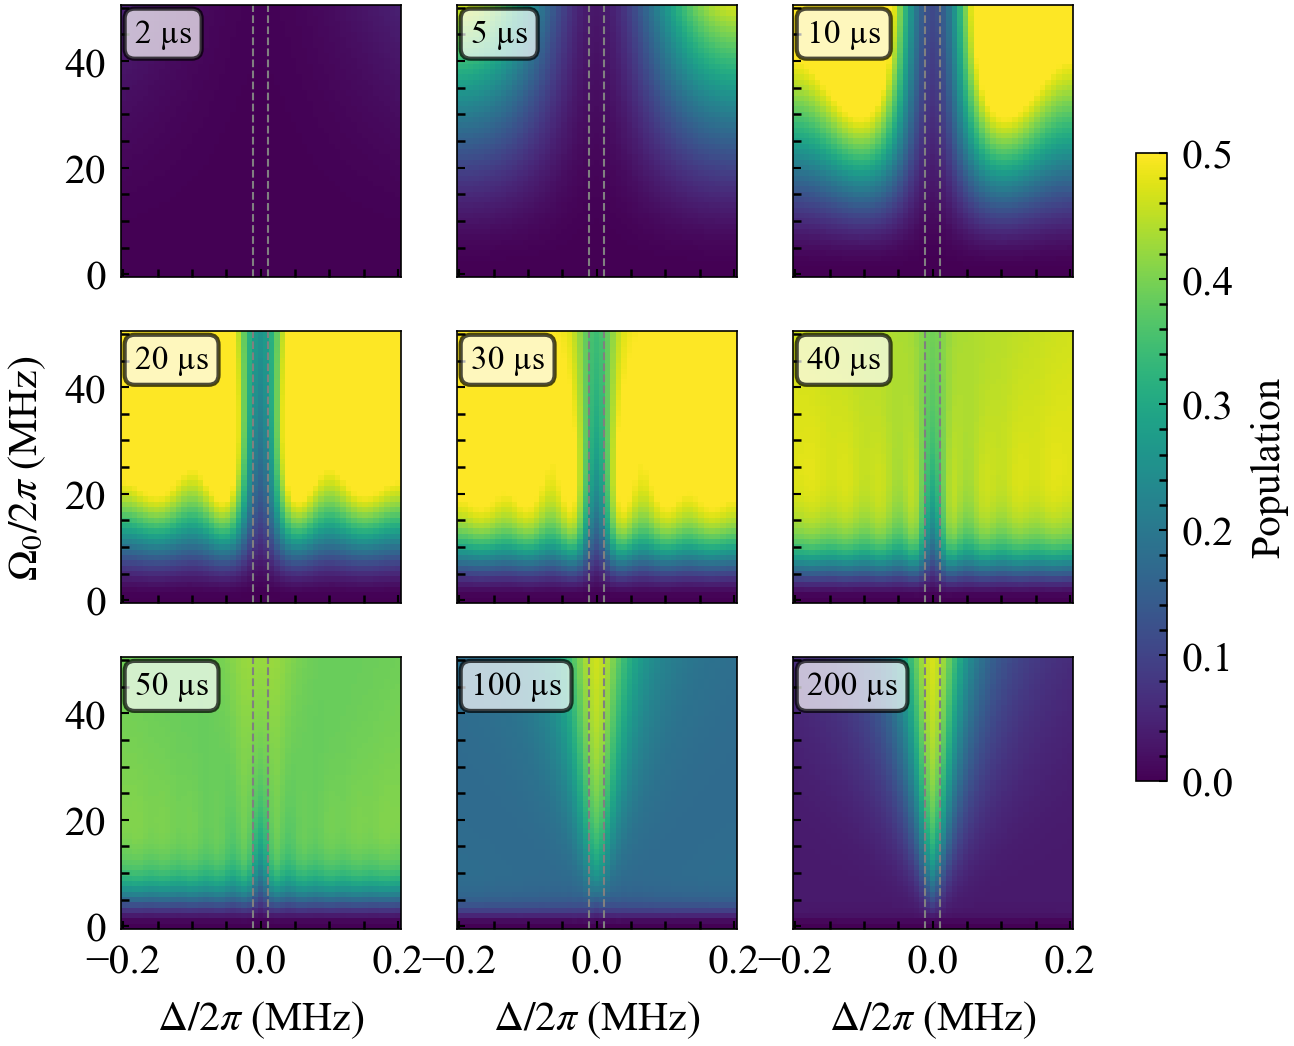
\includegraphics[width=1\linewidth]{figures/spectroscopy_length_comparison.png}
    \caption{Numerical spectroscopic response obtained using echo–root–Lorentzian pulses for different pulse durations (indicated in each panel). As the pulse length increases, the spectral linewidth progressively narrows, approaching the decoherence-limited resolution set by the coherence time $T_2$. For pulse durations comparable to or exceeding the relaxation time $T_1$, population decay during the interrogation leads to an elevated off-resonant background, reducing spectral contrast despite the continued narrowing of the resonance feature.}
    \label{fig:fig8}
\end{figure}




Replacing the inequality in Eq.  (\ref{eq:adiabatic-condition}) with an equality provides a approximate boundary condition between adiabatic  and non-adiabatic regions
\begin{equation}
   \sqrt{\Omega^2(t_0) + \Delta_b^2}= \frac{\Delta_b\dot{\Omega}(t_0)}{2[\Delta^2+\Omega^2(t_0)]}
,\end{equation}
where $t_0$ denotes the time at which the non-adiabatic coupling $| \dot{\vartheta}|$, is maximal, and  $\Delta_b$  marks the boundary between the adiabatic and non-adiabatic regimes. This condition allows us to extract a threshold value for the detuning range $\Delta<\Delta_b$ which marks the range of detunings where post-pulse excitation remains significant. The excitational linewidth scales proportionally to the threshold detuning  $\text{FWHM}\propto\Delta_b$. Consequently, we are particularly interested in the functional dependence of $\Delta_b$ on the peak Rabi frequency $\Omega_0$. 




